\clearpage
\markboth{Problem 5}{Problem 5: Part 3}

\textbf{Problem Statement:} Implement and analyze the Ridders' method for solving the equation $f(x) = 0$. For guidance, you might wish to read the Wikipedia page on the Ridders' method. Also feel free to consult other sources.

\subsection*{Brief Description of the method}

Given the initial bracketing interval $[x_0, x_2]$, containing \textbf{one} solution, and such that $f(x_0)$ and $f(x_2)$ have opposite signs, compute the midpoint $x_1 = (x_0 + x_2)/2$. Then define a new function $h(x) = f(x)e^{ax}$. Find the parameter $a$ that ensures $h(x_1) = \frac{1}{2}(h(x_0) + h(x_2))$. Then define $x_3$ as the $x$-intercept of the line passing through $(x_0, h(x_0))$ and $(x_2, h(x_2))$. Use $x_3$ as one of the endpoints of the next interval bracketing the solution. The other endpoint is $x_1$ if $f(x_1)f(x_3) < 0$. Otherwise, choose either $x_0$ or $x_2$ based on the requirement that the sign of $f(x)$ at the chosen point must be opposite to the sign of $f(x_3)$. Continue until the desired accuracy is reached.

\subsection*{Part 3}
\addcontentsline{toc}{subsection}{Problem 5.3}

Implement Ridders' method on a computer together with the standard bisection method for finding \textbf{all} solutions of
$$e^x - x^2 = 0.$$

\noindent\rule{\textwidth}{0.4pt}

\vspace{1em}

\textbf{Solution:}

First I'll plot the graph of $e^x - x^2$ to identify the intervals where the function changes sign, indicating the presence of roots.

% Graph: Zoomed In
\begin{figure}[h!]
    \centering
    \begin{minipage}[t]{0.48\textwidth}
        \centering
        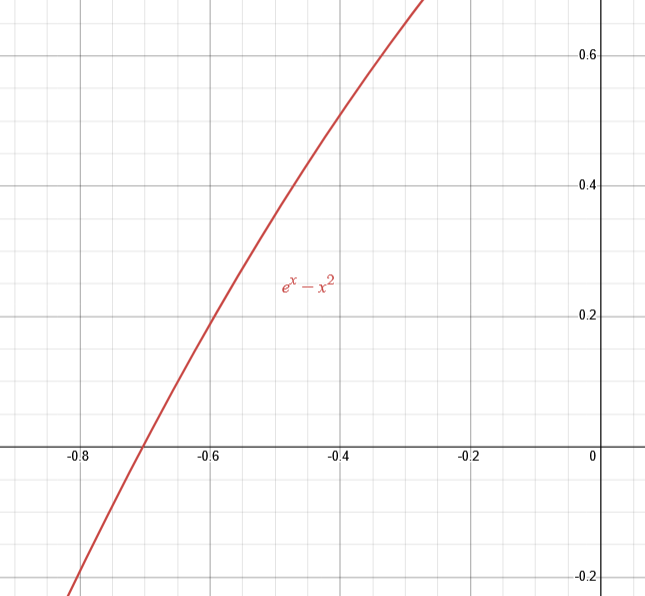
\includegraphics[width=\linewidth]{figures/p05-3-graph-of-ex-x2-zoomed-in.png}
    \end{minipage}%
    \hfill
    \begin{minipage}[t]{0.48\textwidth}
        \centering
        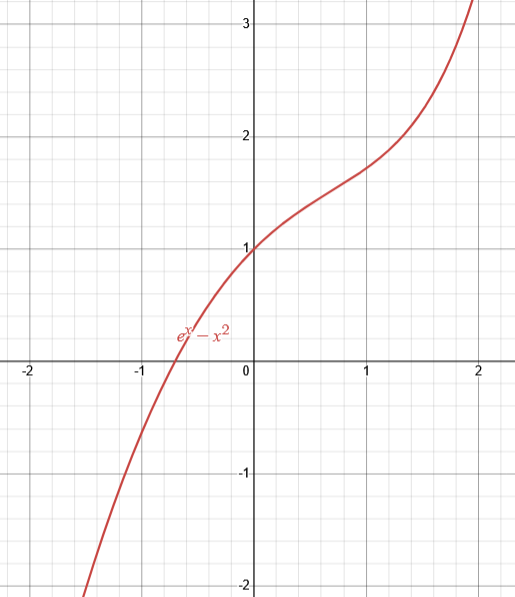
\includegraphics[width=\linewidth]{figures/p05-3-graph-of-ex-x2-zoomed-out.png}
    \end{minipage}
    \caption{Graphs of $e^x - x^2$: We can see from the zoomed in graph on the left that there is a single root in $[\text{-}0.8,\,\text{-}0.6]$. The zoomed out graph on the right shows that the function is monotonically increasing and has no other zeros.}
    \label{fig:ex-x2-side-by-side}
\end{figure}

From \Cref{fig:ex-x2-side-by-side}, it can be seen that there is one root in the interval $[\text{-}0.8,\,\text{-}0.6]$. Since $f(x)<0$ for $x=\text{-}0.8$ and $f(x)>0$ for $x=\text{-}0.6$, I can use this interval to find the root using both the bisection method and Ridders' method.

\subsubsection*{Root Finding on the Original Interval}

For the purpose of \textbf{root finding}, I applied both methods to the smaller interval $[\text{-}0.8,\,\text{-}0.6]$ with tolerances $\epsilon = 10^{-5}$ and $\delta = 10^{-5}$. The results are shown in \Cref{fig:combined-output}.

\begin{figure}[h!]
    \centering
    
\includegraphics[width=0.9\textwidth]{"figures/p05-3-bisection-and-ridders-methods-outputs-on-ex-x2.png"}
    \caption{Terminal output comparing root finding results for $e^x - x^2$ using both Ridders' method and bisection method on the interval $[\text{-}0.8,\,\text{-}0.6]$. Ridders' method converged in just 1 iteration, while bisection required 12 iterations to achieve similar accuracy.}
    \label{fig:combined-output}
\end{figure}

As shown in \Cref{fig:combined-output}, Ridders' method found the root $x = \text{-}0.703468627463942$ with $|f(x)| \approx 2.29 \times 10^{-6}$ in only \textbf{1 iteration}, while the bisection method required \textbf{12 iterations} to find $c = \text{-}0.703466796875000$ with $|f(c)| \approx 1.19 \times 10^{-6}$. This dramatic difference in iteration count demonstrates the superior efficiency of Ridders' method even on a relatively small interval.

The full code for the Ridders' method function is provided in Appendix~\ref{appendix:p05-3-code}. The bisection code is not shown here, as it was implemented in Homework 1 and is a subset of the Ridders' approach.

\vspace{2em}
\noindent\rule{\textwidth}{0.4pt}
